\documentclass[11pt]{elsarticle}

\usepackage{graphicx}
\usepackage{amssymb}
\usepackage{amsmath}
\usepackage{caption}
\usepackage{lineno}
\usepackage{subcaption}





\makeatletter
\def\ps@pprintTitle{%
 \let\@oddhead\@empty
 \let\@evenhead\@empty
 \def\@oddfoot{\centerline{\thepage}}%
 \let\@evenfoot\@oddfoot}
\makeatother

\begin{document}

\begin{frontmatter}

\title{Modelling Predator Prey Systems Using C}

\author{Daniel Bromley - 400106329}

\address{PHYSICS 2G03: Scientific Computing}



\end{frontmatter}

\section*{Introduction}

The aim of this project is to successfully model a predator-prey system. This will entail observing how the populations of both the predator and prey may vary with time and how each population in turn affects the other. The Lotka-Volterra equations will be the mathematical principles underpinning this model. These equations are the basis for simulating a predator-prey system, and consist of a pair of first order, non-linear, differential equations. The populations change with time, this is illustrated mathematically in equations 1 and 2 $^{[1]}$.

\begin{equation}
\dot{x}\left ( x,y \right )=\alpha x - \beta xy
\end{equation}
\begin{equation}
\dot{y}\left ( x,y \right )=\delta xy - \gamma y
\end{equation}
Where $x$ is the population of prey, $y$ is the population of predators, $\dot{x}$ and $\dot{y}$ represents the rate of change of the populations with respect to time, $\alpha$ is the growth rate of the prey in the absence of interaction with predators, $\beta$ measures the impact of predation on $\dot{x}$ against $x$, $\gamma$ is the death rate of the predators in absence of interaction with the prey and $\delta x$ denotes the net rate of growth of the predator population in response to the size of the prey population. Equations 1 and 2 are quite simple and therefore rely on a few assumptions. It is assumed that the prey has enough food and therefore does not compete with regards to food, thus the death/birth rates of the population are not affected. The only source of food for the predator population is the prey population, thus, if the prey population is affected, the repercussions of this are felt by the predator population. The rate of change of the population is proportional to its size. In nature, hunting is not often very successful, therefore animals tend to eat a lot in a small amount of time and can often go long periods without food. This would be difficult to model, therefore we presume that predators can eat an unlimited amount and are always successful hunters. Another important assumption is that during the process the environment does not change in favour of one species, and also neither species is able to genetically adapt to certain conditions. Based on these assumptions, it can be deduced that this model is not completely realistic in modelling a real life predator-prey system. Thus, in later parts of the project, terms of a higher polynomial order may be added to these equations in order to take into account real life scenarios, i.e. one prey becomes diseased, a natural disaster affects both populations etc. The adjusted Lotka-Volterra equations take the form of equations 3 and 4 $^{[2]}$:

\begin{equation}
\dot{x}\left ( x,y \right )=\alpha x - \beta xy - \kappa x^2
\end{equation}
\begin{equation}
\dot{y}\left ( x,y \right )=\delta xy - \gamma y - \lambda y^2
\end{equation}
Where $\kappa$ represents the effect of the environment on the prey population. This value may be positive for a damaging effect i.e. disease, natural disaster, competition for food etc. or it may be negative for a beneficial effect i.e. abundance of food, good health and high reproduction rates etc. $\lambda$ is the effect of environment on the predator population. Again, this value may be positive for a damaging effect or it may be negative for a beneficial effect for reasons discussed above.

\subsection*{\textbf{Runge-Kutta Method}}

As the Lotka-Volterra equations are first order, non-linear, differential equations, they cannot be solved directly when using computer code. They therefore have to be solved iteratively. In order to achieve this, we employ the Runge-Kutta method. This is an iterative method that yields the approximate solutions for ordinary differential equations, like the Lotka-Volterra equations. The most common member of the Runge-Kutta set is known as the `RK4' method. The RK4 method is illustrated in equations 5 through 9 $^{[3]}$:

\begin{equation}
k_1=hf\left ( x_n,y_n \right )
\end{equation}
\begin{equation}
k_2=hf\left ( x_n+\frac{K_{x1}}{2},y_n+\frac{K_{y1}}{2} \right )
\end{equation}
\begin{equation}
k_3=hf\left ( x_n+\frac{K_{x2}}{2},y_n+\frac{K_{y2}}{2} \right )
\end{equation}
\begin{equation}
k_4=hf\left ( x_n+k_{x3},y_n+k_{y3} \right )
\end{equation}
\begin{equation}
a_{n+1}=a_n + \frac{1}{6}\left (k_1+2k_2+2k_3+k_4  \right )
\end{equation}
Where $f\left ( x_n,y_n \right )$ is either $\dot{x}\left ( x,y \right )$ or $\dot{y}\left ( x,y \right )$, $h$ is the iteration step, which in this case is the time interval $dt$ and $a$ is either $x$ or $y$. The initial $x$ and $y$ values i.e. the initial population values are entered into the equations, hence the overall effect of $\dot{x}$ and $\dot{y}$ on $x$ and $y$ over a time interval $dt$ are represented by equation 9. Each $k$ interval plays a specific role in finding the new $x$ and $y$ values. $k_1$ is the increment due to the beginning of the interval, $k_2$ is the increment due to the midpoint of the interval, $k_3$ is another increment due to the midpoint of the interval and $k_4$ is the increment due to the end of the interval. By taking the average of the 4 $k$ values and subsequently adding it to the previous $x$ or $y$ value, the new population level is returned. This value has a greater weight at the midpoint, thus yielding a more accurate result.

\section*{Program and Results}
In order to model the predator prey system, both the Lotka-Volterra equations and the Runge-Kutta method were implemented in conjunction with one another. This was done via the use of the  computer programming language C. The code that produces the values for the populations at each time interval is seen in appendix 1. In order to understanding the values returned by the code, the populations are graphed against time. The population values are then also plotted against each other, as this will signify the evolution of each population with respect to each other, and is therefore useful in determining how stable (or unstable) a system is. The computing language python was used to produce the graphs, as the matplotlib.pyplot library found in python is a more effective way of producing easily understandable and aesthetically pleasing plots. This python code can be found in appendix 2.

In order to validate the c code and determine the data it returns is of worth, predetermined values for the $\alpha,\beta,\delta,\gamma$ coefficients and the initial population values were used. These were derived from actual data taken on the populations of the Canadian lynx and snowshoe hares over the years spanning from 1900 to 1920 in the boreal forests of North America $^{[4]}$. The results of this data and the coefficients it produces can be seen in figure 1.

\begin{figure}
\centering
   \begin{subfigure}[b]{1\textwidth}
   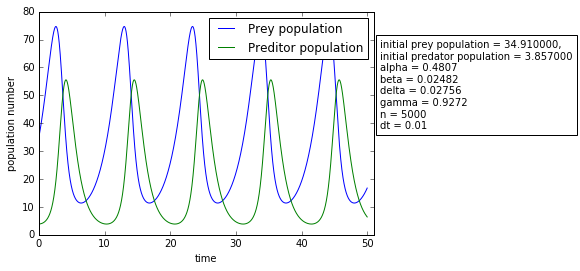
\includegraphics[width=0.9\linewidth]{figure1_time.png}
   \caption{}
   \label{fig:Ng1} 
\end{subfigure}

\begin{subfigure}[b]{1\textwidth}
   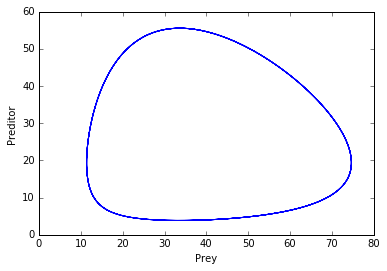
\includegraphics[width=0.6\linewidth]{figure1_phase.png}
   \caption{}
   \label{fig:Ng2}
\end{subfigure}

\caption{(a) Note that the non-integer population values are those extrapolated from the lynx-hare data $^{[4]}$. (b) The phase diagram shows a complete loop, thus the system is in stable state}
\end{figure}
\noindent
\newline
Figure 1 (a) successfully demonstrates the predator-prey system of the lynx-hare. Real life characteristics of a predator prey system can be seen in figure 1 (a), a good example of such characteristics is the phase difference observed between the minima and maxima with respect to each population. This difference is as a result of a culmination of reasons; as the prey population begins to grow the predator population has more to eat and thus also grows, there comes a point to which the prey population reaches a maximum, as there is only a finite source of food. Thus, the population diminishes due to lack of food. Despite this, the predator population continues to increase as the recent bountiful food supplies allow the predators to reproduce more. Thereafter, the repercussions of a decrease in the prey population is felt as the predators have less to eat, and thus they too begin to decrease in numbers. After some time the prey population hits a minimum. Here there is plenty of food for the prey as the preys numbers are lower, enabling them to begin to reproduce again. Subsequently, the prey levels increase and the cycle repeats itself. The system exhibits almost harmonic oscillatory motion. From this we can deduce that it is a stable system. Consequently, as our results agree with predictions, we are therefore able to infer that the code is reliable in producing correct outcomes. This is further illustrated in fig 1 (b) by the shape of the phase diagram: as it is a single loop with no ends it can therefore be deduced that the system is stable, again agreeing with predictions. Another way to test the codes credibility is to set one of the populations to a fixed point, in this case the prey population has been fixed. Therefore, the Lotka-Volterra equations dictate that the predator populations should increase exponentially, as seen in equation 10.
\begin{equation*}
\dot{x}=0\therefore x = constant
\end{equation*}
\begin{equation*}
\dot{y}=\delta xy -\gamma y
\end{equation*}
\begin{equation*}
\frac{dy}{y}=\left(\delta x-\gamma\right)dt
\end{equation*}
\begin{equation}
\therefore y=Ae^{\left(\delta x -\gamma\right)t}
\end{equation}
Where $A$ is some unknown integration constant, $\delta$ and $\gamma$ are the specified constants, $x$ is the prey population which in this case is constant and $t$ is the time the system has been allowed to evolve.

\begin{figure}
\centering
   \begin{subfigure}[b]{1\textwidth}
   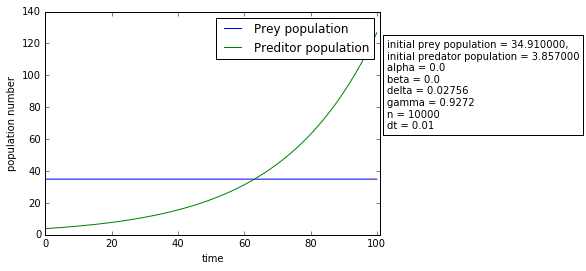
\includegraphics[width=0.90\linewidth]{figure2_time.png}
   \caption{}
   \label{fig:Ng1} 
\end{subfigure}

\begin{subfigure}[b]{1\textwidth}
   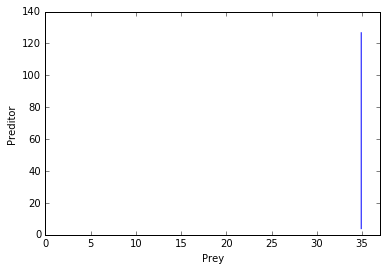
\includegraphics[width=0.59\linewidth]{figure2_phase.png}
   \caption{}
   \label{fig:Ng2}
\end{subfigure}

\caption{(a) Note that the lynx-hare values were kept constant apart from making $\alpha$ and $\beta$ equal to zero. (b) The phase diagram yields a straight line, thus the prey population remained constant whilst the predator population increased, as predicted }
\end{figure}

It can be seen in figure 2 (a) that the $\alpha$ and $\beta$ constants were set to zero, thus rendering the prey population at a constant level. This produced an exponentially increasing predator population, as predicted by equation 10. Figure 2 (b) further demonstrates the constant prey population and the increasing predator population. As the code simulates the expected scenarios for both the lynx-hare data and the fixed point system, we can therefore conclude that its calculations are correct, thus allowing us to further explore the codes modelling capabilities. 
\newline

The previous models have assumed that the environment does not change in favour of one species, and also neither species genetically adapts to certain conditions i.e. there is no disease, natural disaster, lack of food, inter-population competition etc. This results in a model that isn't efficient at simulating real life systems effectively. Concerning the resolution of this discrepancy, equations 3 and 4 are implemented in the code instead of equations 1 and 2. In order to allow a fair comparison between the results of each model, the same initial populations and $\alpha,\beta,\delta,\gamma$  coefficients are used as those in the previous models. The $\kappa$ and $\lambda$ coefficients are given values, thus yielding a predator-prey model that is biased towards a specific population.

\begin{figure}
\centering
   \begin{subfigure}[b]{1\textwidth}
   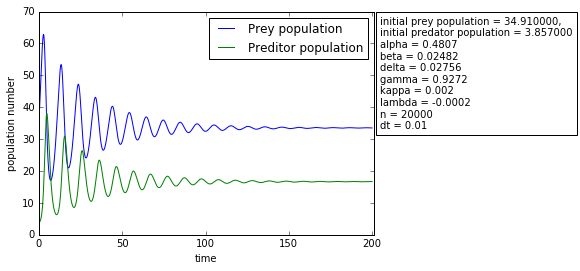
\includegraphics[width=0.9\linewidth]{figure3_time.png}
   \caption{}
   \label{fig:Ng1} 
\end{subfigure}

\begin{subfigure}[b]{1\textwidth}
   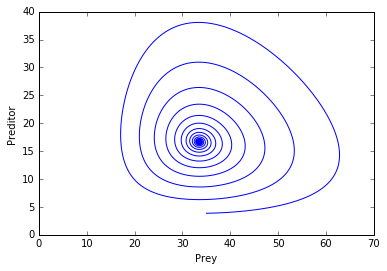
\includegraphics[width=0.60\linewidth]{figure3_phase.png}
   \caption{}
   \label{fig:Ng2}
\end{subfigure}

\caption{(a) This model represents that of a biased one, in this case it is biased in favour of the predator, this is represented by the positive $\kappa$ and negative $\lambda$ values (b) This phase diagram unlike the others, spirals to a point, thus yielding a system that becomes almost constant in terms of population levels  }
\end{figure}

It can be seen in figure 3 (a) that the $\kappa$ and $\lambda$ constants were made to be positive and negative respectively, thus simulating an environment/event that favours the predators. These extra terms consequently produced a system that resembles a damped harmonic oscillator. This result is not very intuitive, but can be explained somewhat; as the coefficients aren't very large, the bias is only slightly towards the predators. Thus, the overall size of the prey is slowly decreased with every cycle to the point at which the system becomes stable, and the effect of the bias takes no effect on either the prey or the predator. Figure 3 (b) further illustrates the system entering into a constant population level, as represented by the predator-prey phase diagram spiralling to a single point. Upon further inspection of the data produced for this system, the final values of the populations were found to be 33.50 for the prey and 16.7 for the predators (please note it is understood that these are non-integer values, however it is unimportant when trying to obtain a general outlook of the model and can thus be ignored). Therefore, the model was successful in being biased towards the predators as their population increased from 3.9 to 16.7, and the preys population decreased from 34.9 to 33.5.
\newpage
\subsection*{\textbf{Further investigation}}
So as to render a deeper understanding and produce a more successful simulation of real life predator prey systems seen in nature, there are a few avenues one could explore. One of these is the introduction of more than one predator or prey to the system, as seen in nature, real ecosystems often contain many predators and many preys, all interlinked. This would be achieved by  using the Lotka-Volterra equations for $n$ species. These are a set of more complex equations, that take into account the effect of more species by employing matrices. Another subject to examine more closely could be to make the Lotka-Volterra coefficients ($\alpha,\beta,\delta,\gamma$ etc.) time dependent. This would be more accurate in representing issues like disease and food shortages, as these problems do not last indefinitely, thus their effect on the population changes with time. This may be achieved using a Monte Carlo system in order to predict whether an event will occur or not, based on its probability.


\section*{Conclusion}
By implementing the Lotka-Volterra equations for predator-prey models, in conjunction with the Runge-Kutta iterative method and the computing language `c', a successful computer simulation for predator-prey systems was produced. The results of the code were validated using coefficients taken from actual predator-prey data based on that of the Canadian lynx and snowshoe hare. The code was further tested by fixing the population of the prey to a constant number and then comparing it to the analytical solution of the Lotka-Volterra equations. These findings illustrated the competency and effectiveness of the code. Merits of the Runge-Kutta method are its speed when implemented via computer code, its simplicity and its accuracy, as the Runge-Kutta method, especially the ‘RK4’ method, is efficient in producing accurate results.



\newpage

\section*{References}

\noindent
\sloppy
[1] - Lotka, A. J. (1920).\underline{Analytical note on certain rhythmic relations in}
\newline
\underline{ organic systems}. Proc. Natl. Acad. Sci. 6, 410-415.
\newline
\newline
\noindent
\sloppy
[2] - Sternberg, S. (2009).\underline{Lotka-Volterra}. Available: http://www.math.harvard.edu/library/sternberg/slides/11809LV.pdf. Last accessed November 2016
\newline
\newline
\noindent
[3] - Abramowitz, M., and Stegun, I.A. (1964). \underline{Handbook of Mathematical Functions}. Applied Mathematics Series, Volume 55
\newline
\newline
\noindent
[4] - Mahaffy, J.M. (2000).\underline{Lotka-Volterra Models}.Available: http://jmahaffy.sdsu.edu/courses/f09/math636/lectures/lotka/qualde2.html. Last accessed November 2016
\newline
\newline
\noindent




\newpage
\appendix
\subsection{C code}
\begin{verbatim}
#include <stdio.h>
#include <stdlib.h>

double alpha = 0.4807, beta = 0.02482, delta = 0.02756, 
			gama = 0.9272, kappa = 0.000, 
			lambda = 0.000; //these can be changed 
			in order to produce specific scenarios

double dxdt(double x, double y){
	
	return alpha*x-beta*x*y-kappa*x*x;
	
}

double dydt(double x, double y){

	return delta*x*y-gama*y-lambda*y*y;

}

void RK(double dt, double *px, double *py){

	double	kx1,
		ky1,
		kx2,
		ky2,
		kx3,
		ky3,
		kx4,
		ky4,
		A[2],x=*px,y=*py;

		kx1=dt*dxdt(x,y);
		ky1=dt*dydt(x,y);
		kx2=dt*dxdt(x+kx1/2,y+ky1/2);
		ky2=dt*dydt(x+kx1/2,y+ky1/2);
		kx3=dt*dxdt(x+kx2/2,y+ky2/2);
		ky3=dt*dydt(x+kx2/2,y+ky2/2);
		kx4=dt*dxdt(x+kx3,y+ky3);
		ky4=dt*dydt(x+kx3,y+ky3);
		x = x + (1.0/6.0)*(kx1 + 2*kx2 + 2*kx3 + kx4);
		y = y + (1.0/6.0)*(ky1 + 2*ky2 + 2*ky3 + ky4);
	
  		*px = x;
  		*py = y;
	
}

int main(){

	FILE * fp;
	int i, n=5000;
	float dt = 0.01;
	double x = 34.91, y = 3.857;

	fp = fopen("output.txt", "w");
	fprintf(fp, "number of steps is: %d\n", n);
	fprintf(fp, "time interval is: %f\n", dt);
	fprintf(fp, "initial prey pop: %f, initial predator population: 
	%f\n", x,y);
	fprintf(fp, "alpha = $%$f beta = %f delta = %f gamma = %f 
	kappa = %f lambda = %f\n", alpha,beta,delta,gama,kappa,lambda);
	fprintf(fp, "x pop, y pop, time\n");

	for(i=0;i<=n;i++){
	RK(dt, &x, &y);
	fprintf(fp,"\%f \%f \%f\n", x, y, dt*i);
	
	}

}

\end{verbatim}
\newpage
\subsection{Python code}
\begin{verbatim}
import numpy as np
import matplotlib.pyplot as plt
import sys

filename = "output.txt" #this can be changed for 
				      different files
def datacollector(filename):
    if filename.endswith(".txt"): 
        pass
    else:
        sys.exit("filetype not txt")
    try:
        with open(filename, "r") as datafile:
            
            data = np.genfromtxt(datafile,delimiter=" ",
            skip_header=5,filling_values="nan")
        
    except IOError:
        sys.exit("There has been an issue locating the 
        file - "{}" - please check file is in correct location"
        							.format(filename))

    return data

def constantfinder(filename):
    with open(filename, "r") as file:
        lines = [line.split() for line in file]
        consts = lines[3]

    alpha = float(consts[2])
    beta = float(consts[5])
    delta = float(consts[8])
    gamma = float(consts[11])
    kappa = 0.0
    lambd = 0.0
    for i in consts: 
        if i == "kappa" or i == "lambda":
            kappa = float(consts[14])
            lambd = float(consts[17])
        
    
    return alpha, beta, delta, gamma, kappa, lambd

def initialpop(filename):
    with open(filename, "r") as file:
        lines = [line.split() for line in file]
        initpop = lines[2]

    prey = initpop[3]
    pred = initpop[7]

    return prey, pred

def timeint(filename):
    with open(filename, "r") as file:
        lines = [line.split() for line in file]
        timeint = lines[1]
        nint = lines[0]

        n = nint[4]
        dt = float(timeint[3])

    return dt, n

xpop = datacollector(filename)[:,0]
ypop = datacollector(filename)[:,1]
t = datacollector(filename)[:,2]
alpha, beta, delta, 
gamma, kappa, lambd = constantfinder(filename)
dt, n = timeint(filename)
prey, pred = initialpop(filename)
txt = "initial prey population = {}\ninitial predator population 
= {}\nalpha = {}\nbeta = {}\ndelta = {}\ngamma = {}\nkappa 
= {}\nlambda = {}\nn = {}\ndt = {}".format(prey,pred,alpha,
beta,delta,gamma,kappa,lambd,n,dt)

if float(kappa) == float(0.0) and float(lambd) == float(0.0):
    txt = "initial prey population = {}\ninitial predator 
    population = {}\nalpha = {}\nbeta = {}\ndelta = {}\ngamma 
    = {}\nn = {}\ndt = {}".format(prey,pred,alpha,beta,delta,
    gamma,n,dt)



plt.plot(t, xpop, label = "Prey population")
plt.plot(t, ypop, label = "Preditor population")
plt.legend(loc="upper right")
plt.xlim(0,t[len(t)-1]+1)
a = plt.ylim(0)
plt.text(((t[len(t)-1]+1)*1.02),a[1]/2.1,txt,
	    bbox=dict(facecolor="none", edgecolor='black'))
plt.ylabel("population number")
plt.xlabel("time")
plt.show()

plt.plot(xpop,ypop)
plt.ylabel("Preditor")
plt.xlabel("Prey")
plt.ylim(0)
plt.xlim(0)
plt.show()

\end{verbatim}


\end{document}